\documentclass{scrreprt}
\usepackage[english]{babel}
\usepackage[T1]{fontenc}
\usepackage{lmodern}
\usepackage{blindtext}
\usepackage[utf8]{inputenc}
\usepackage{siunitx} %For unit handling%
\renewcommand{\familydefault}{\sfdefault}
\newcommand{\unit}[1]{\ensuremath{\, \mathrm{#1}}}
\usepackage{amssymb, amsmath, cancel, ulem, graphicx, float, tabularx, multirow, bm}
\usepackage{amsmath}
\usepackage{caption}
\usepackage{subcaption}
\usepackage{mathtools}
\usepackage{tikz}
\newcommand*\circled[1]{\tikz[baseline=(char.base)]{
            \node[shape=circle,draw,inner sep=1pt] (char) {#1};}}
\renewcommand{\phi}{\varphi}

\setcounter{secnumdepth}{5}
\setcounter{tocdepth}{5}

\author{Urs Gerber\\09-921-156 \and Gian-Luca Mateo\\11-113-545}
\date{11th of March 2013}

\title{Lenses}
\subtitle{Practical course report}

\begin{document}

\maketitle

\tableofcontents
\newpage

\chapter{Experiment: Lenses}

\section{Introduction}

\subsection{Goal of the experiment}
The goal of this experiment is to determine the focal distance of a set of lenses using the method proposed by German scientist Friedrich Wilhelm Bessel.

\subsection{Theory}

\subsubsection{Lens equation}
The commonly known lens formula is
\begin{equation}
\frac{1}{f} = \frac{1}{g} + \frac{1}{b}
\end{equation}
where $f$ is the focal distance, $g$ is the object distance and $b$ is the image distance.

\subsubsection{Lens pair}
The lens equation for a pair of lenses $L_1$ and $L_2$ looks a bit different:
\begin{equation}
\frac{1}{f}= \frac{1}{f_1} + \frac{1}{f_2} - \frac{d}{f_1 \cdot f_2}
\end{equation}
where $f_i$ is the focal distance of lens $L_i$ and $d$ is the distance between $L_1$ and $L_2$

\subsubsection{Bessel's method}
We use the method proposed by Bessel to find the focal distance $f$ of a lens by experimental means. Let $a \doteq g + b$ be a fixed quantity. Then there exists for a given focal distance $f < \frac{a}{4}$ only two possible lens positions which produce a sharp image $B$ of object $G$. 

\begin{figure}[H]
	\centering
  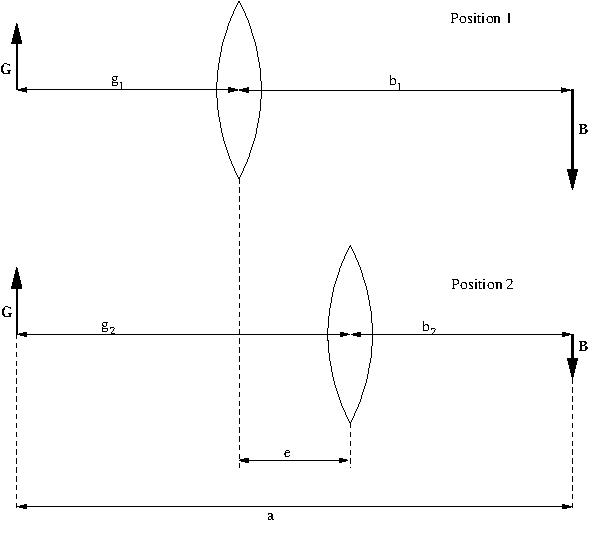
\includegraphics[width=0.9\textwidth]{diag/lens_skript.pdf}
	\caption{Finding focal distance using Bessel's method}
	\label{fig:method}
\end{figure}

These lens positions are given by
\begin{equation}
b_{1,2} = \frac{a}{2} \pm \sqrt{\left(\frac{a}{2}\right)^2-a\cdot f}
\end{equation}

\begin{equation}
g_{1,2} = a-b_{1,2}=b_{2,1} = \frac{a}{2} \mp \sqrt{\left(\frac{a}{2}\right)^2-a\cdot f} 
\end{equation}

\begin{equation}
b_1 - b_2 = 2 \cdot \sqrt{\left(\frac{a}{2}\right)^2-a\cdot f}
\end{equation}

Using $e \doteq b_1 - b_2$ and solving for $f$ yields

\begin{equation}
\boxed{f = \frac{a^2-e^2}{4\cdot a}}
\end{equation}

\paragraph{Diverging lenses}
The image of a diverging lens ($f_z < 0$) is virtual and thusly cannot be projected onto a screen. To measure the focal distance $f_z$ we just use a second lens with known focal distance $f_s$ and we get
\begin{equation}
\frac{1}{f} = \frac{1}{f_s} + \frac{1}{f_z} - \frac{d}{f_s \cdot f_z}
\end{equation}
and hence
\begin{equation}
f_z = \frac{f \cdot \left( f_s - d\right)}{f_s - f}
\label{lenssystem}
\end{equation}

\paragraph{Lenses with large focal distances}
It is not possible to directly measure focal distances $f > \frac{a}{4}$. Analogous to diverging lenses we just use a second lens with known focal distance $f_s$ to calculate the large focal distance $f_x$

\begin{equation}
f_x = \frac{f \cdot \left( f_s - d\right)}{f_s - f}
\label{lenssystem2}
\end{equation}

\subsubsection{Preliminary exercises}

\textbf{Task 1}
\begin{equation}
	f=18cm\quad G=46cm\quad B=1cm
\end{equation}
\begin{equation}
	b=f\frac{B+G}{G}=18.391cm
\end{equation}
\begin{equation}
	g=f\frac{B+G}{B}=846cm
\end{equation}
\\
\textbf{Task 2}
\begin{equation}
	f=5cm\quad b=6cm
\end{equation}
\begin{equation}
	g=\frac{bf}{b-f}=30cm
\end{equation}
\\
\textbf{Task 3}
\begin{equation}
	G=30cm\quad g=500cm\quad B=1cm
\end{equation}
\begin{equation}
	f=\frac{gB}{B+G}=16.129cm
\end{equation}
\textbf{Task 4}
\begin{figure}[H]
	\centering
  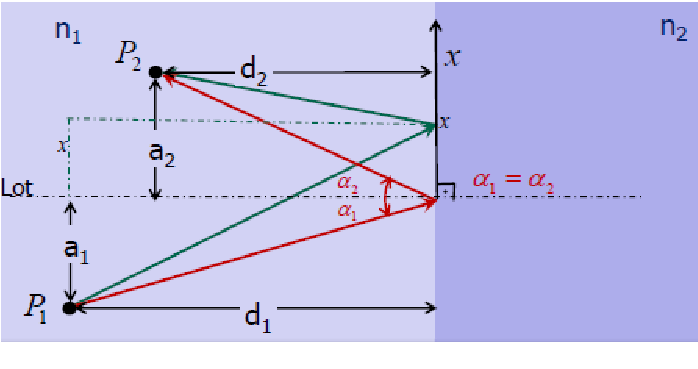
\includegraphics[width=0.9\textwidth]{diag/exercises1.pdf}
	\caption{law of reflection}
\end{figure}
\begin{equation}
\sum n_i s_i \stackrel{!}= \mbox{Minimum}
\end{equation}
\begin{equation}
\Rightarrow n_1 \sqrt{(a_1+x)^2+d_1^2}+n_1\sqrt{(a_2-x)^2+d_2^2} \stackrel{!}= \mbox{Minimum}
\end{equation}
\begin{equation}
\Rightarrow \frac{d}{dx} \left(\sqrt{(a_1+x)^2+d_1^2}+\sqrt{(a_2+x)^2+d_2^2}\right) \stackrel{!}= 0
\end{equation}
\begin{equation}
\frac{1}{2} \frac{2(a_1+x)}{\sqrt{(a_1+x)^2+d_1^2}}+\frac{1}{2} \frac{-2(a_2-x)}{\sqrt{(a_2-x)^2+d_2^2}} \stackrel{!}= 0
\end{equation}
\begin{equation}
\frac{(a_1+x)^2}{(a_1+x)^2+d_1^2} = \frac{(a_2-x)^2}{(a_2-x)^2+d_2^2}
\end{equation}
This obviously holds for $x=0 \Rightarrow x=0$ satisfies the minimum condition.
\\ \\
Law of refraction:
\begin{figure}[H]
	\centering
  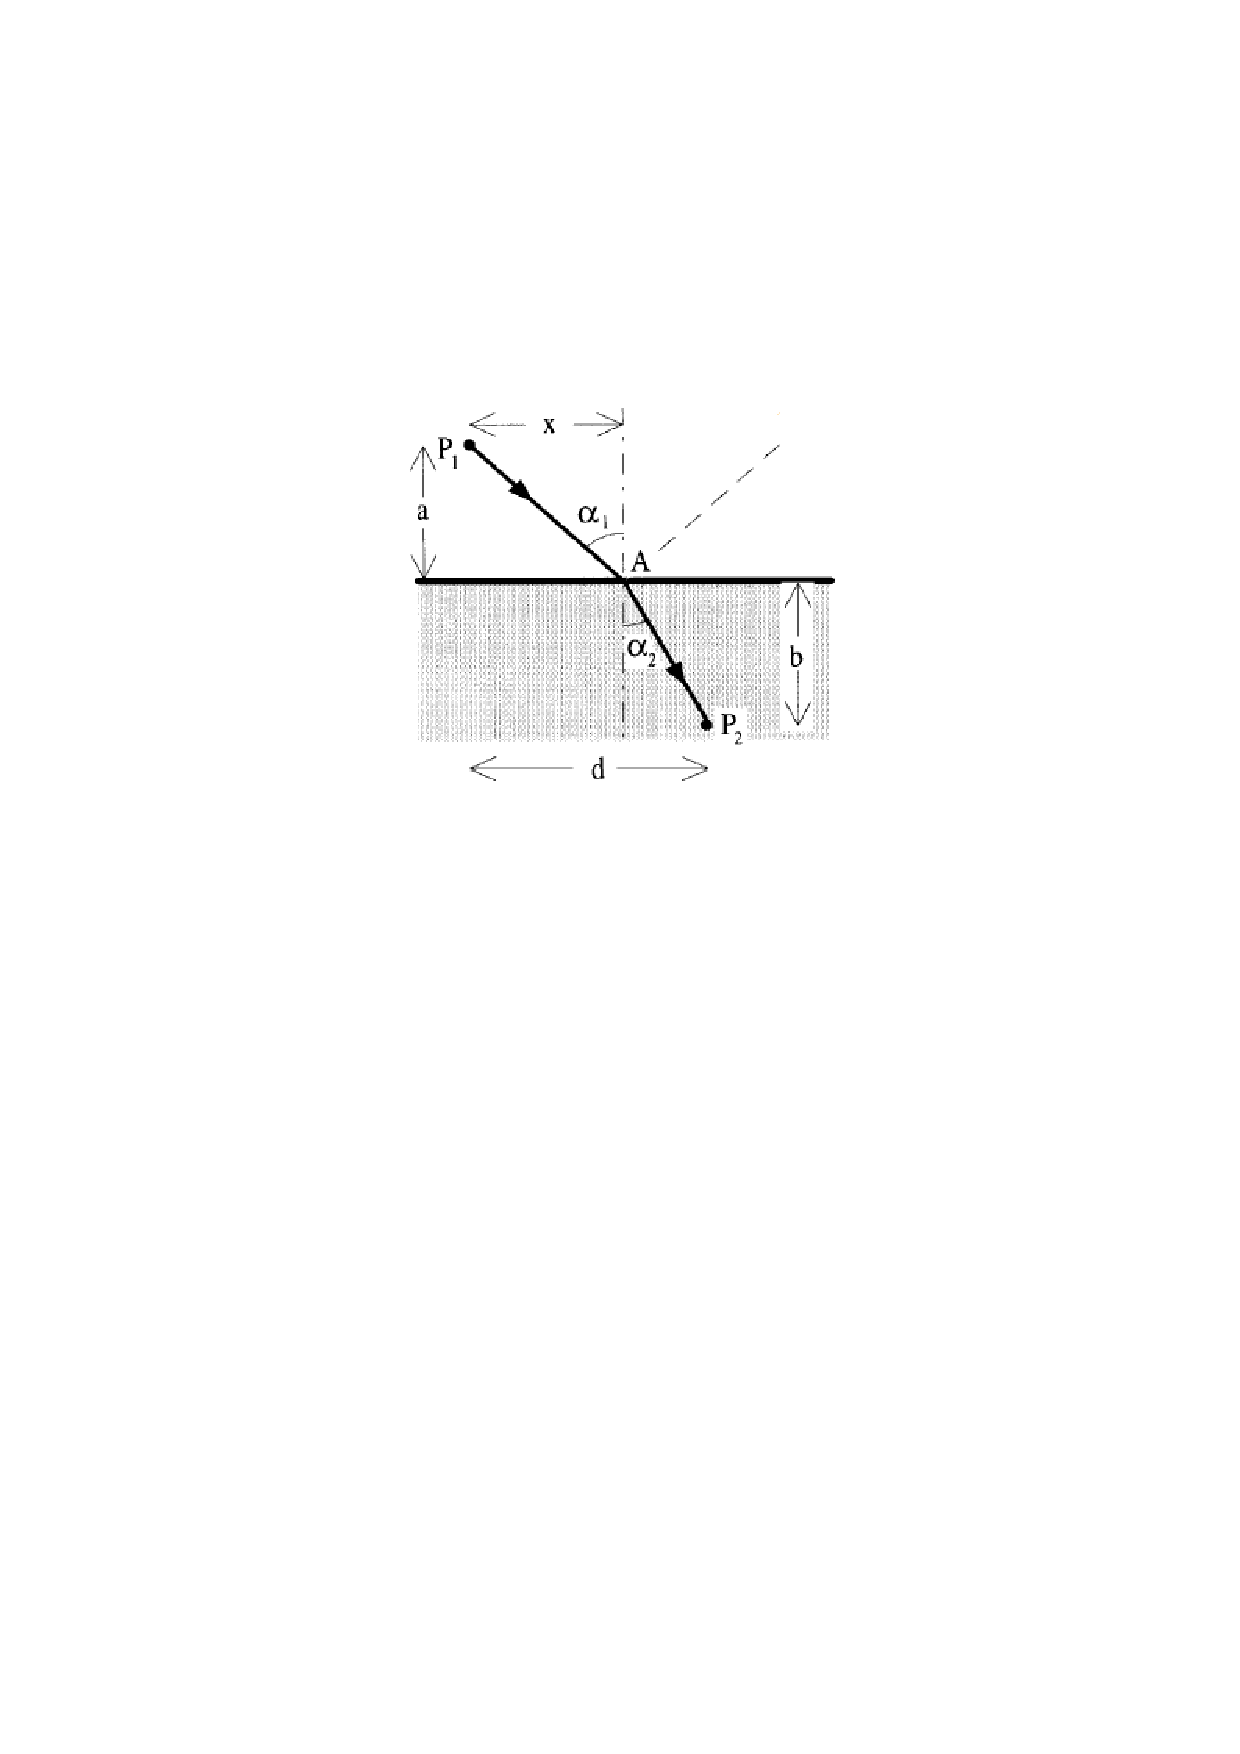
\includegraphics[width=0.5\textwidth]{diag/exercises2.pdf}
	\caption{Law of refraction}
\end{figure}
\begin{equation}
s(x) = n_1 \cdot \overline{P_1 A} + n_2 \cdot \overline{A P_2} = n_1 \cdot \sqrt{a^2+x^2} + n_2 \cdot \sqrt{b^2+(d-x)^2} \stackrel{!}= \mbox{Minimum}
\end{equation}
\begin{equation}
\frac{ds}{dx} = n_1 \cdot \frac{x}{\underbrace{\sqrt{a^2+x^2}}_{\sin \alpha_1}}- n_2 \cdot \frac{d-x}{\underbrace{\sqrt{b^2+(d-x)^2}}_{\sin \alpha_2}} \stackrel{!}= 0
\end{equation}
\begin{equation}
\Rightarrow \frac{\sin \alpha_1}{\sin \alpha_2}=\frac{n_2}{n_1}
\end{equation}
\\ 
\textbf{Task 5}\\
\begin{figure}[H]
	\centering
  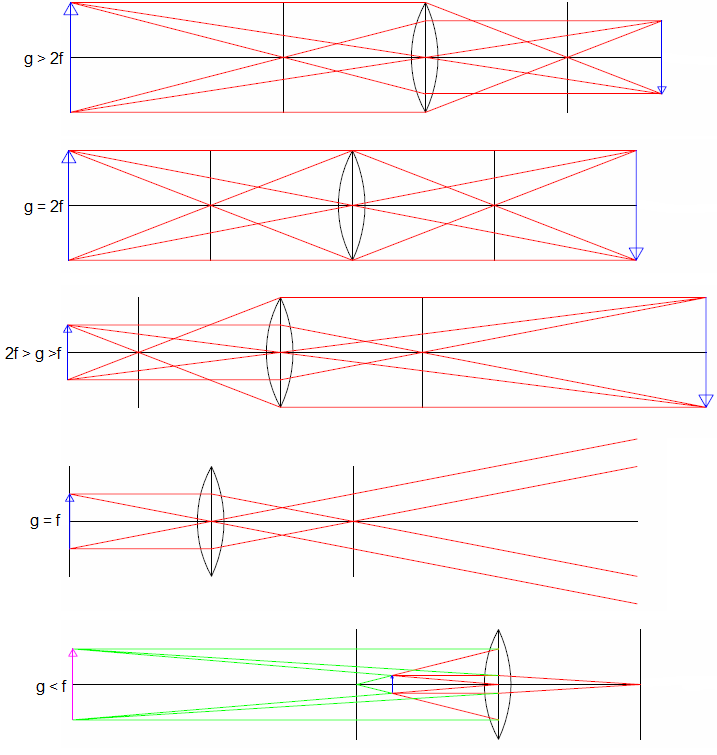
\includegraphics[width=0.9\textwidth]{diag/exercises3.png}
	\caption{Task 5}
\end{figure}
\textbf{Task Chapter 11.2.3}
\begin{equation}
f = \frac{a^2-e^2}{4a} = \frac{600^2-255.3^2}{4\cdot 600}mm = 122.84mm
\end{equation}
\begin{equation}
f_x = \frac{f \cdot (f_s-d)}{f_s-f} = \frac{122.84\cdot (80-10)}{80-122.84}mm = -200.71mm
\end{equation}

\subsection{Uncertainty analysis}

\begin{align*}
b_1 &= a - x_1\\
b_2 &= a - x_2\\
\end{align*}
\[e = b_1 - b_2 = \lvert x_2 - x_1 \rvert\]
\begin{equation}
\Longrightarrow s_e^2 = s_{x_1}^2 + s_{x_2}^2
\end{equation}

\paragraph*{Directly measured $f$}
For directly measured lenses with $0 < f < \frac{a}{4}$ the standard error of the mean $s_f$ is
\[
f = \frac{a^2-e^2}{4\cdot a}
\]

\begin{equation}
\Longrightarrow s_f^2 = \left[ \frac{1}{2} - \frac{a^2-e^2}{4 a^2} \right]^2 \cdot s_a^2 + \frac{e^2 \left( s_{x_1}^2 + s_{x_2}^2 \right)}{4  a^2}
\end{equation}

\paragraph*{Indirectly measured $f_z$} For indirectly measured lenses with $f_z < 0$ or $f_z > \frac{a}{4}$ and known focal distance $f_s$ of the second lens the standard error of the mean $s_{f_z}$ is

\[f_z = \frac{f \cdot \left( f_s - d\right)}{f_s - f}\]


\begin{equation}
\xRightarrow{d \; \approx \; 0} s_{f_z}^2 = \frac{f_s^4\cdot s_f^2 + f^4 \cdot s_{f_s}^2}{\left( f-f_s \right)^4}
\end{equation}

\section{Experiment setup and execution}

\subsection{Used materials}
The materials used in this experiment are the following:
\begin{itemize}
\item a projector which projects a static image
\item a milk glass screen
\item a rail with imprinted scale
\item 4 different lenses, labelled 1C to 4C
\item Some mounts for attaching all of the above to the rail
\end{itemize}
\subsection{Assembly}
For our measurements, the screen is attached at one end of the rail and the projector at the other, facing the screen. In between, a lens is placed and its position varied until two points are found where a sharp image appears on the screen. If we found no positions, we attached a second lens to the first lens and repeated the measurement. This whole process is repeated 5 times for each lens.

\section{Measurements}

\begin{figure}[H]
	\centering
  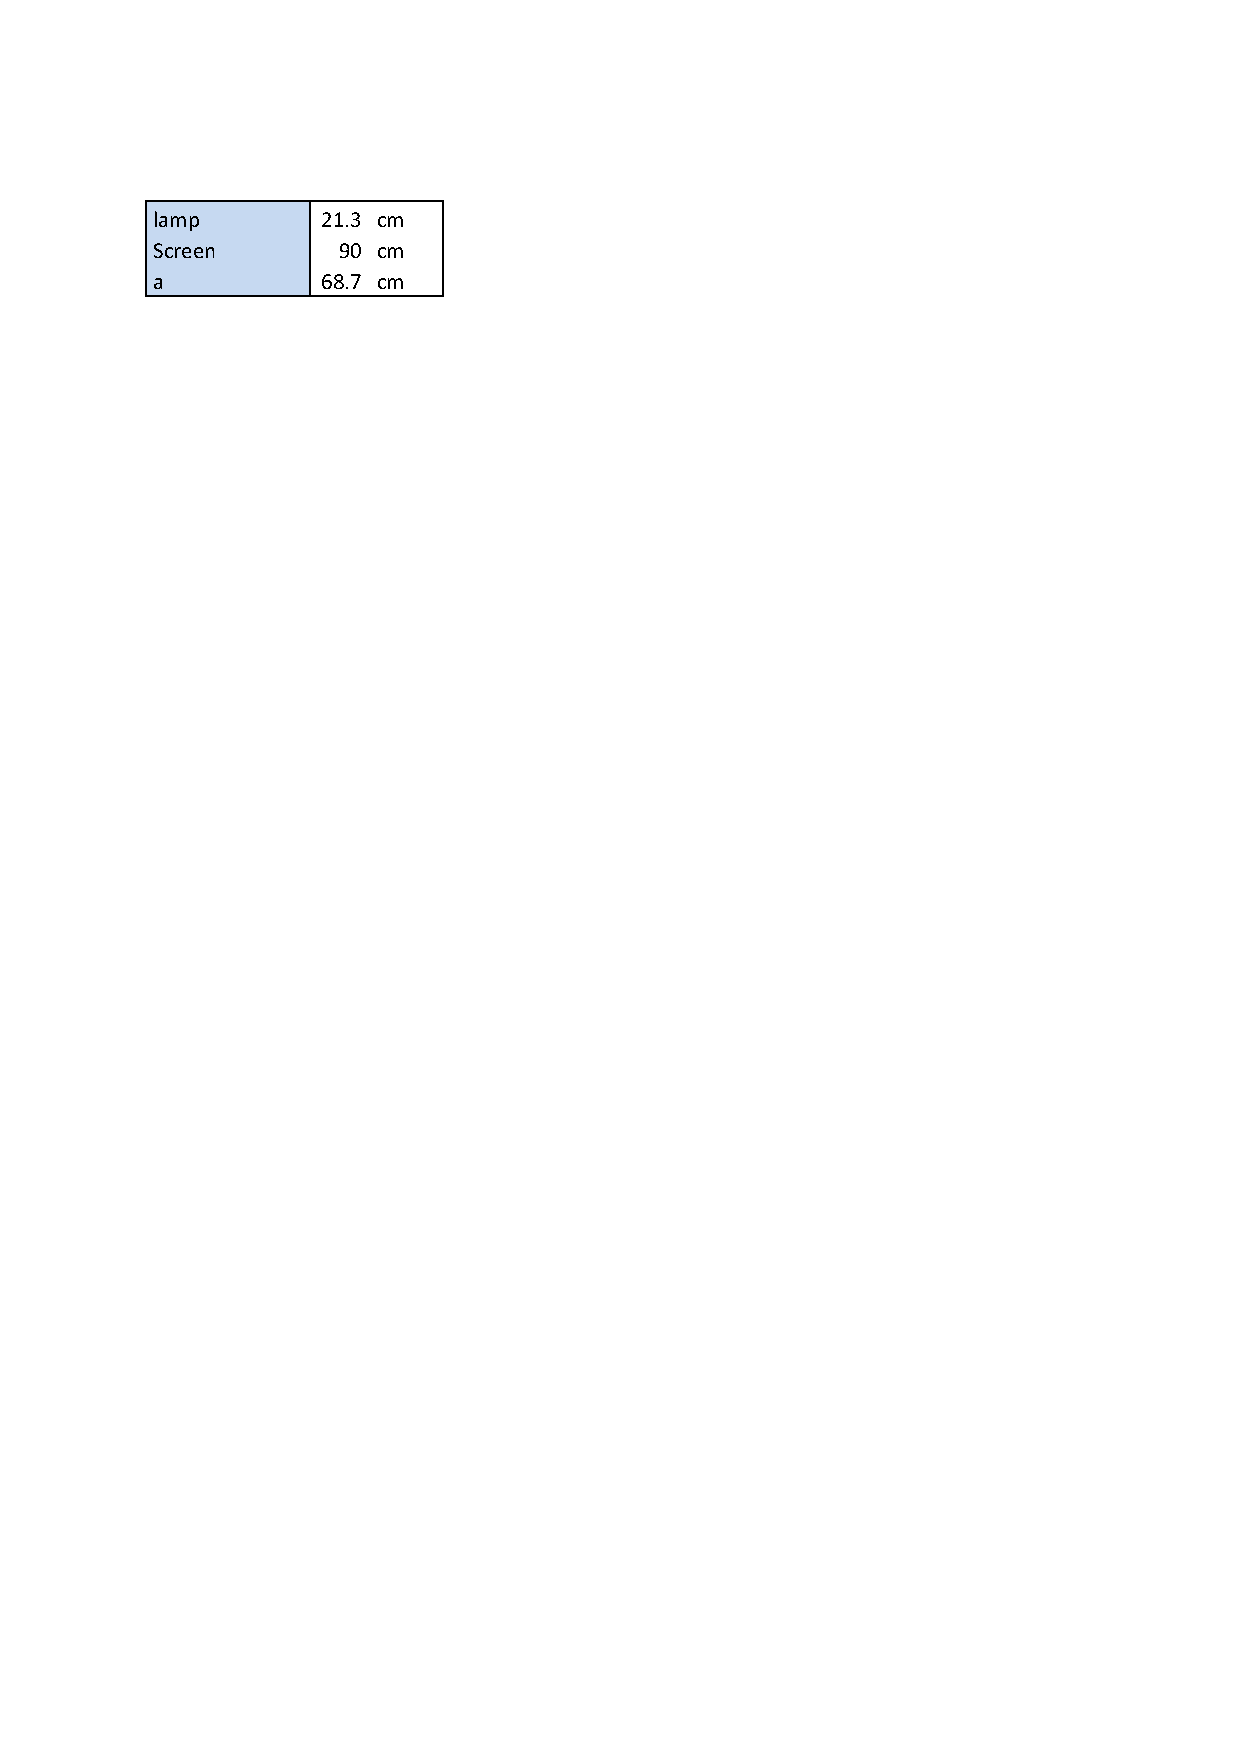
\includegraphics[width=0.4\textwidth]{diag/general_measurements.pdf}
	\caption{General measurements for our assembly}
\end{figure}

\begin{figure}[H]
        \centering
        \begin{subfigure}[b]{0.3\textwidth}
                \centering
                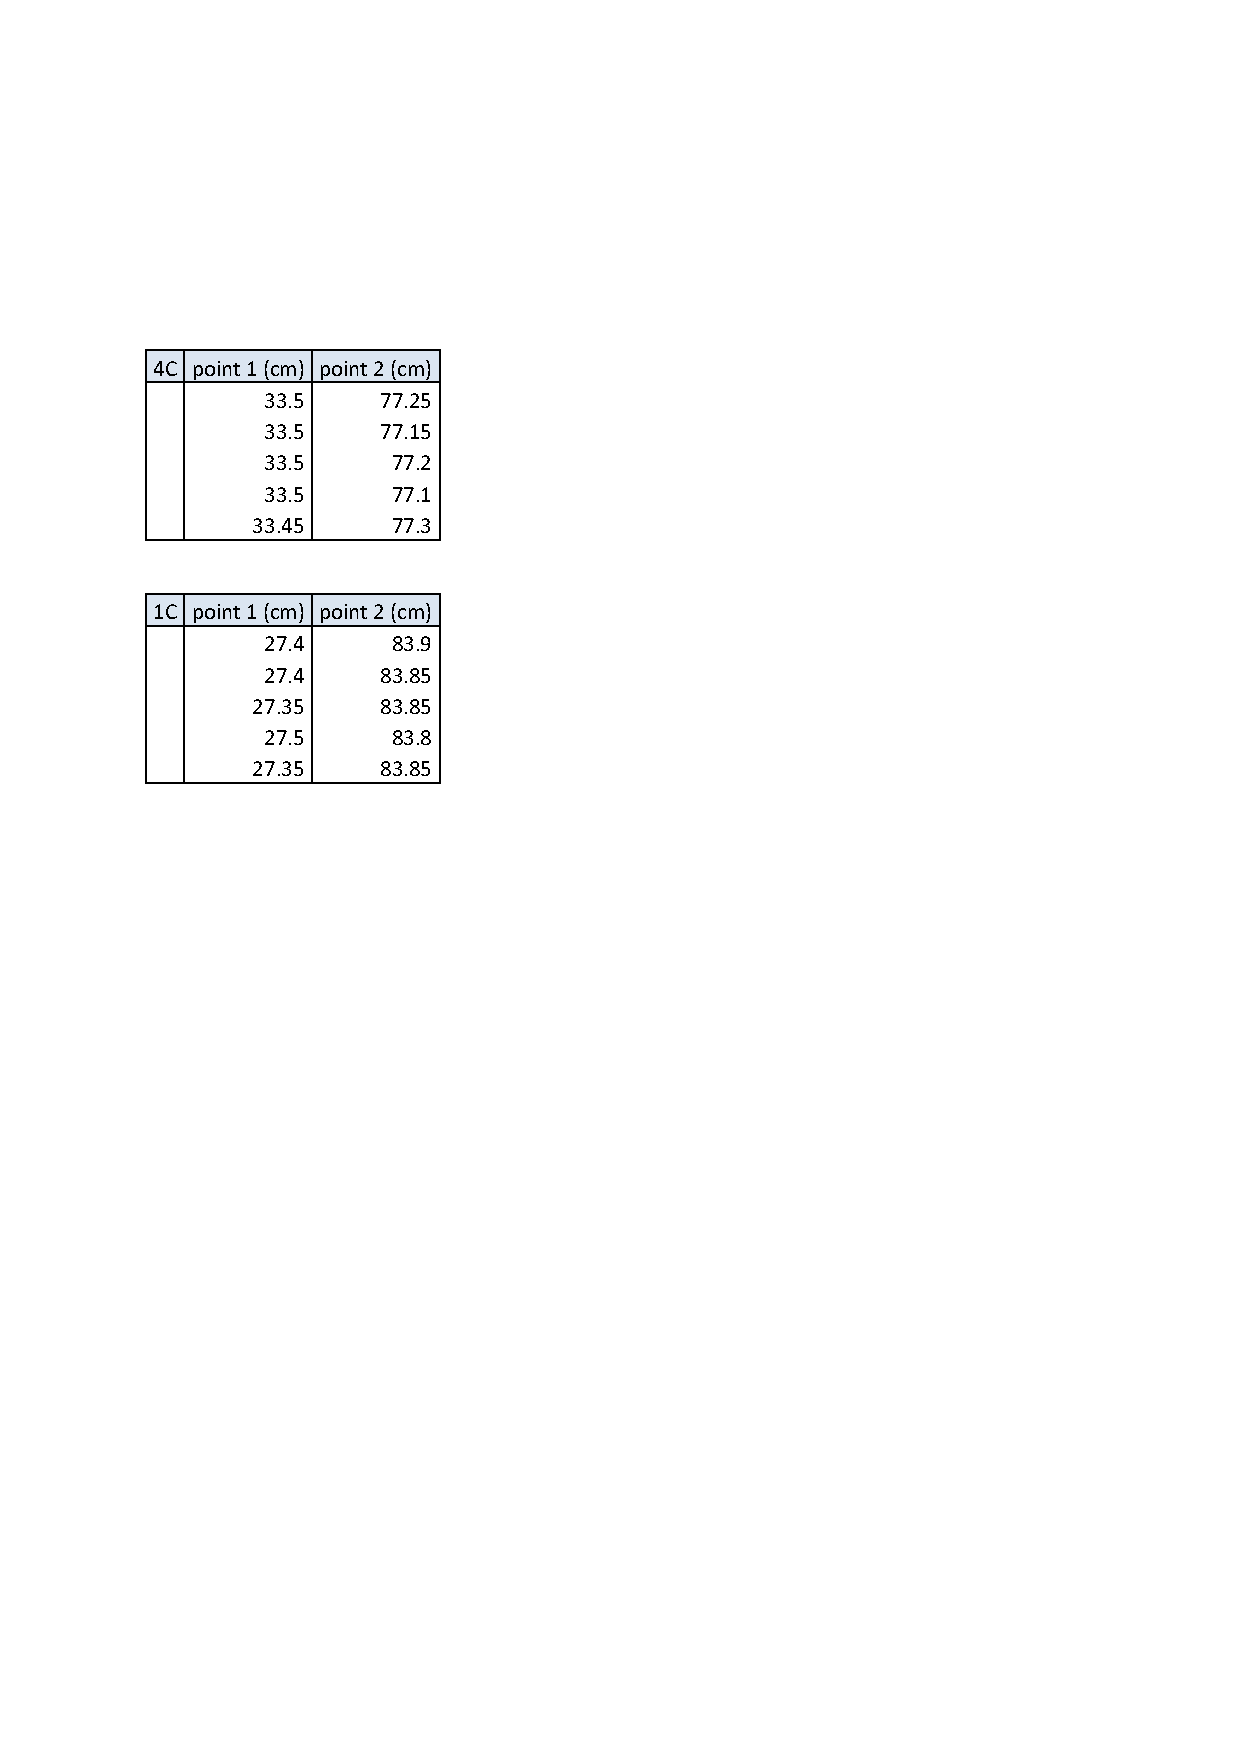
\includegraphics[width=\textwidth]{diag/one_lens.pdf}
                \caption{Lenses measured directly}
                \label{fig:direct}
        \end{subfigure}%
        ~
        \begin{subfigure}[b]{0.345\textwidth}
                \centering
                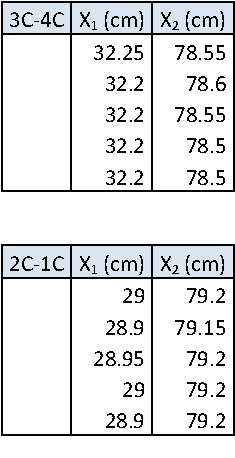
\includegraphics[width=\textwidth]{diag/two_lenses.pdf}
                \caption{Lenses measured indirectly}
                \label{fig:indirect}
        \end{subfigure}
        \caption{Measurements of lens positions $X_1$ and $X_2$}
        \label{fig:measurements}
\end{figure}

\section{Analysis and Discussion}

\begin{equation}
x_i = X_i - x_{lamp} (= g_i)
\end{equation}
\begin{table}[H]
\center
\begin{tabular}{|l|c|c|c|c|}
\hline
Lens(-es) & $x_1$ [cm] & $x_2$ [cm] & $\sigma_{x_1}$ [m] & $\sigma_{x_2}$ [m]\\
\hline
1C &$12.19 \pm 0.0274$&$55.9 \pm 0.0354$& $0.0612$ & $0.0354$\\
2C-1C &$28.95 \pm 0.0224$&$57.89 \pm 0.01$&$0.05$&$0.0224$\\
3C-4C &$10.91 \pm 0.01$&$57.24 \pm 0.0187$&$0.0224$&$0.0418$\\
4C &$12.13 \pm 0.01$&$55.9 \pm 0.0354$&$0.0224$&$0.0791$\\
\hline
\end{tabular}
\end{table}
Applying the results of our uncertainty analysis to our results -- using $\pm 1$mm as estimated error for $a$ -- and using formulae \ref{lenssystem} and \ref{lenssystem2} wherever we had to combine two lenses, assuming the distance $d$ between two lenses is $0$, we get for $f$:

\begin{table}[H]
\center
\begin{tabular}{|l|c|c|c|}
\hline
Lens & $f$ [m] measured & $f$ [m] theoretical & relative error\\
\hline
1C & $ 0.05579 \pm 0.0004278$&$0.05$&$11.58\%$\\
2C & $-0.1849 \pm 0.005127$&$-0.15$&$23.25\%$\\
3C & $ 1.1151 \pm 0.06846 $&$1$&$11.51\%$\\
4C & $0.1022 \pm 0.0003653$&$0.1$&$2.22\%$\\
\hline
\end{tabular}
\end{table} 
Our values for $f$ diverge slightly from the theoretically expected ones. Looking for possible sources of error, we found the following:
\begin{itemize}
\item We used the approximation for infinitely thin lenses
\item We assumed the distance between two lenses (where any) to be 0
\item The projected image was very small for some measurements. Judging when the image was sharp proved difficult.
\item In some cases the image was staying sharp even if the lens was moved along the slider ever so slightly, making it difficult to find the most sharp position.
\end{itemize}
Considering all these sources of error, we think our results are reasonable enough. The lenses which we couldn't measure directly tended to show a larger relative error than the ones we measured directly, which confirms the validity of at least parts of our possible sources of error.
\section{Conclusion}

Conclusively, we think our results -considering the sources of error- prove the .......


\begin{thebibliography}{9}

\bibitem{physcript13}
  Peter Wurz,
  \emph{Anleitung zum Physikpraktikum}
  FS2013

\end{thebibliography}

\end{document}
